\documentclass{article}

\usepackage[hidelinks]{hyperref}
\usepackage[utf8]{inputenc}
%\usepackage[latin1]{inputenc}
%\documentclass[15pt,a4paper]{article}
%\usepackage[latin1]{inputenc}
\usepackage{amsmath}
\usepackage{amsfonts}
\usepackage{amssymb}
\usepackage{amsthm}
\usepackage[titletoc,title]{appendix}
\usepackage[english]{babel}
\usepackage[font= small,format=plain,labelfont=bf,up,textfont=it,up]{caption}
\usepackage{colortbl}
\usepackage{diagbox}
\usepackage{eurosym, placeins}
\usepackage{fullpage,graphicx,textcomp,float,gensymb,wrapfig}
\usepackage{longtable}
\usepackage{makecell}
\usepackage{multicol}
\usepackage{mathrsfs}
\usepackage[numbers]{natbib}
\usepackage{parskip}
\usepackage[detect-all]{siunitx}
\usepackage{subcaption}
\usepackage{tabularx}
\newtheorem{theorem}{Theorem}
\usepackage[colorinlistoftodos]{todonotes}
\usepackage{wasysym}


\newcommand{\HRule}{\rule{\linewidth}{0.5mm}}
\newcommand{\red}[1]{{\color{red}{#1}}}

\usepackage{textcomp} % for a single apostrophe with \textquotesingle

\edef\restoreparindent{\parindent=\the\parindent\relax}
\restoreparindent

\allowdisplaybreaks

\graphicspath{{../}}

\sisetup{range-phrase=--}
\sisetup{range-units=single}

\newcommand{\subfigimg}[3][,]{%
	\setbox1=\hbox{\includegraphics[#1]{#3}}% Store image in box
	\leavevmode\rlap{\usebox1}% Print image
	\rlap{\hspace*{0.9\linewidth}\raisebox{\dimexpr\ht1-1.75\baselineskip}{#2}}% Print label
	\phantom{\usebox1}% Insert appropriate spacing
}



\title{Embedded systems: Assignment 3}
\date{\today}
\author{Sjoerd van der Heijden \\ 10336001}

\begin{document}
	\maketitle
	\tableofcontents
	\pagenumbering{arabic}
	\section{Introduction}
	\par In this document I will show and explain my solutions to the tasks detailed in Assignment 3 of the course Embedded Systems 2018, so buckle up.
	
	\section{Assignment 3.1}
	\par For the first part of this assignment I was tasked to create a Petri net model of a four-way intersection for cars. On this intersection cars are only allowed to drive straight, and they have to give priority to cars on their right. 	Fig.\,\ref{fig:ass3_1} shows my solution for this task, with an example initial token distribution. I use inhibitors to prevent cars from driving as long as there's a car coming from their right, or when a car from the left or right is already on the intersection. Cars from opposite directions may cross the intersection simultaniously.
	\par It is possible for the cars to come into deadlock, when a car from each direction is waiting to cross. I did not solve this, as this is not disallowed by the assignment. In order to solve it, one could add another level of priority, e.g. by adding another event that can be fired when cars are waiting from all directions and no cars are crossing, and results in one or two cars crossing the intersection. In the case of two cars crossing they would have to come from opposite directions to prevent collisions.
	\par I also came up with a solution without needing inhibitors, but since it requires a more deliberate setup and is less intuitive I far prefer my current solution.
	
	\begin{figure}
		\centering
		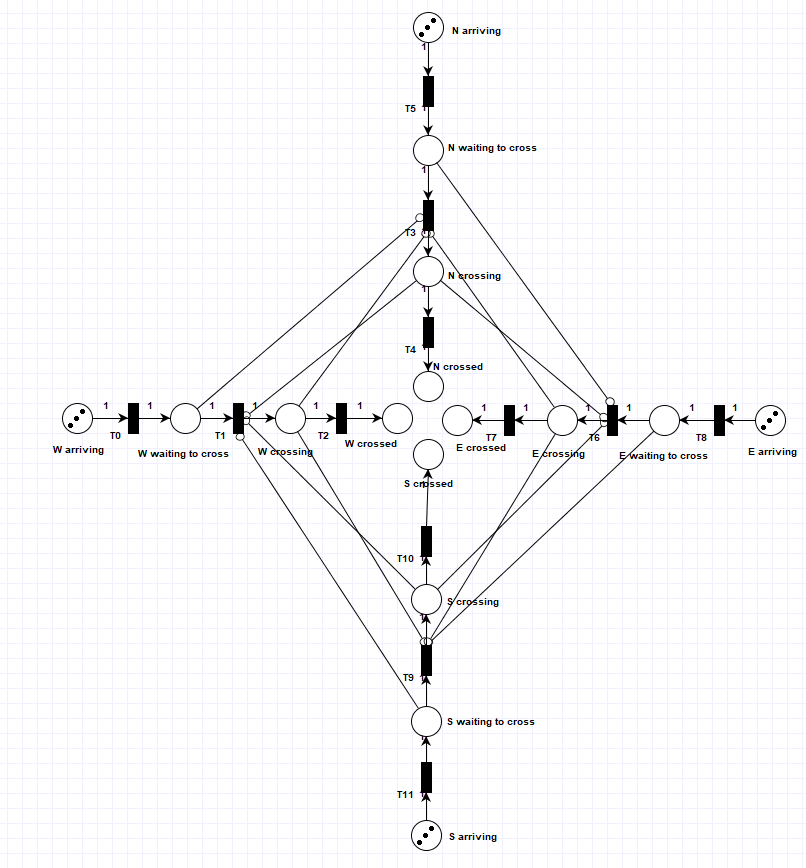
\includegraphics[width=0.8\textwidth]{Ass3_1}
		\caption{My solution to assignment 3.1, this image was created using PIPE 5 \cite{dingle2009pipe2, bonet2007pipe}. The N, E, S and W stand for the cardinal directions. For each direction, a car is first driving towards the intersection (arriving), then reaching the intersection and waiting to cross (waiting), then driving on the intersection (crossing), and finally they leave the intersection (crossed). \label{fig:ass3_1}}
	\end{figure}
	
	
	\section{Assignment 3.2}
	\par The assignment was to compute $Z = A \times \textrm{min}(B, 2\times C)$ using Petri nets. My solution is shown in Fig.\,\ref{fig:ass3_2}. For the sake of being an example, there are tokens present in the net, so that it shows a possible initial state of the aforementioned equation.
	
	\begin{figure}
		\centering
		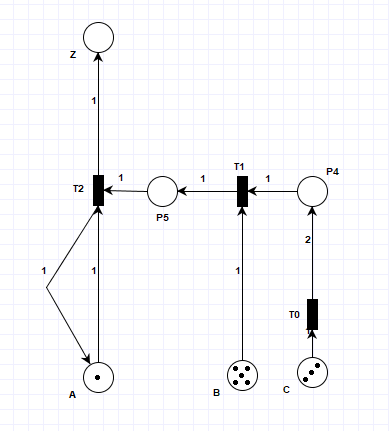
\includegraphics[width=0.5\textwidth]{Ass3_2}
		\caption{My solution to assignment 3.2, this image was created using PIPE 5 \cite{dingle2009pipe2, bonet2007pipe}. \label{fig:ass3_2}}
	\end{figure}
	
	
	\section{Assignment 3.3}
	\par I made a chessclock library in Simulink (see Fig.\,\ref{fig:ass3_3_env} and Fig.\,\ref{fig:ass3_3_chart}), since it had to be the same for both players. How it works is that the players can tell the Simulink chart whose turn it is by toggling a switch. Depending on whose turn it is, one or the other clock starts ticking. When the switch is toggled that clock stops, the local time is reset and global time is incremented, and the other clock starts. After 40 turns both players' clocks are incremented by 15 minutes.
	\par The only downside of having the chessclock implemented as library is that the number of moves taken is measured twice (once in the clock of each player). I set the initial global time to $(60*30) - 15$ in the chart, because I add 15 seconds to the global time before each turn instead of after. In this way they still start with 30 minutes.	
	
	\begin{figure}
		\centering
		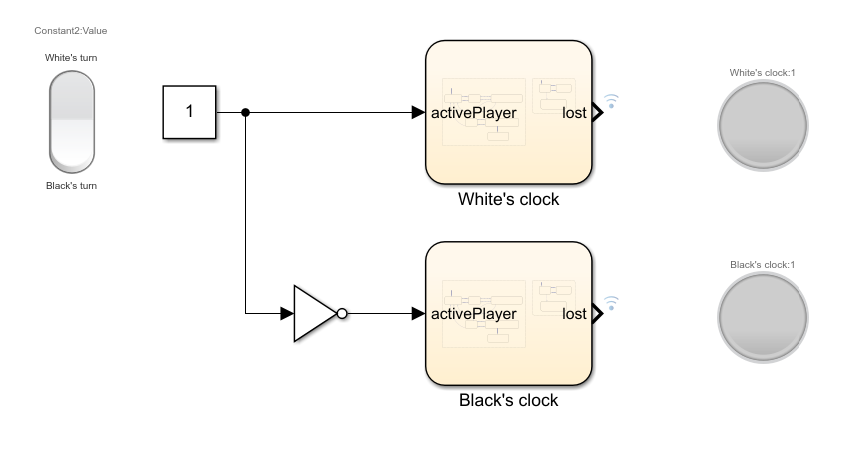
\includegraphics[width=0.5\textwidth]{Ass3_3_environment}
		\caption{The outside view of my solution to assignment 3.3: there is one chess clock for each player, the switch tells which player's turn it is, and the lights are green if a player is still playing and red if a player loses.
		This image was created using PIPE 5 \cite{dingle2009pipe2, bonet2007pipe}. \label{fig:ass3_3_env}}
	\end{figure}

	\begin{figure}
		\centering
		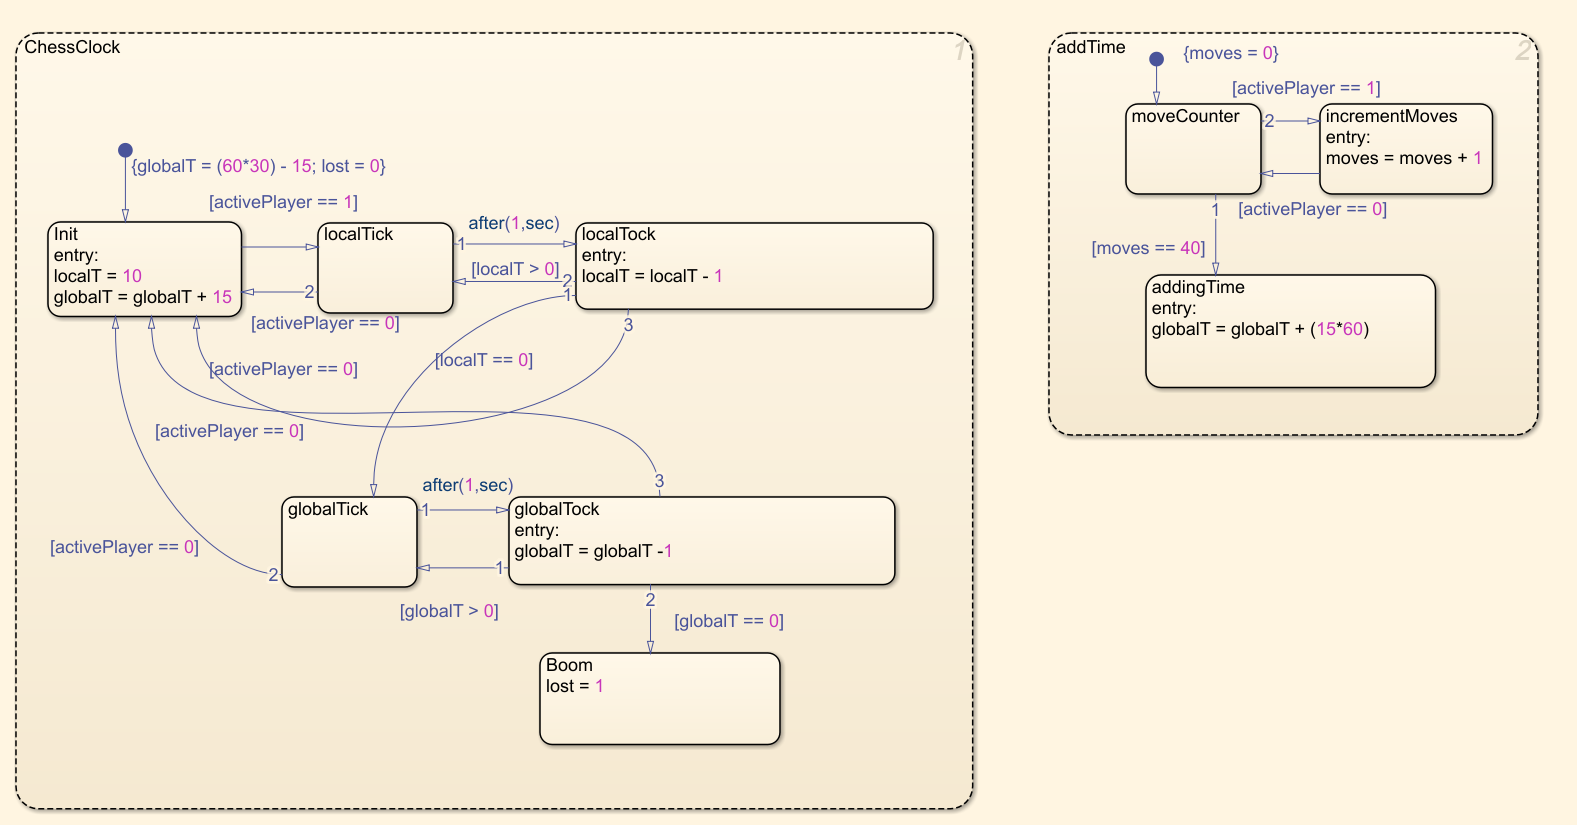
\includegraphics[width=0.8\textwidth]{Ass3_3_chart}
		\caption{A peek under the hood of my chessclock for assignment 3.3. On the left is the chess clock itself, on the right the number of turns taken is logged, and time is added to the clock if 40 turns have passed. The clock itself is somewhat simple: you start with 30 minutes on the global clock, which starts ticking after 10 seconds once it is your turn. After every turn you gain 15 seconds and when the global clock reaches 0 you lose. The clock does not tick during the opponent's turn.
		 This image was created using PIPE 5 \cite{dingle2009pipe2, bonet2007pipe}. \label{fig:ass3_3_chart}}
	\end{figure}
	
	
	\newpage 
	\bibliographystyle{unsrtnat}
	%\bibliographystyle{authordate1}
	\bibliography{bibliography} % The file containing the bibliography
%	\newpage
	

%	\begin{figure}[ht!]
%		\hspace{-2mm}\makebox[\textwidth][c]{
%			\begin{tabular}{@{}p{0.5\linewidth}@{\hspace{5mm}}p{0.5\linewidth}@{}}
%				\subfigimg[width = 0.55\textwidth]{\hspace{0mm}(a)}{Offseteffect} &
%				\subfigimg[width = 0.55\textwidth]{\hspace{0mm}(b)}{RCeffect}
%		\end{tabular}}
%	\end{figure}
		
	
\end{document}
